% --------------------------------------------------------------------------
% Template for WASPAA-2019 paper; to be used with:
%          waspaa17.sty  - WASPAA 2019 LaTeX style file, and
%          IEEEbib.bst - IEEE bibliography style file.
%
% --------------------------------------------------------------------------

\documentclass{article}
\usepackage{waspaa17,amsmath,graphicx,url,times}
%\usepackage{waspaa17,amssymb,amsmath,graphicx,times,url}
\usepackage{color}

% Example definitions.
% --------------------
\def\defeqn{\stackrel{\triangle}{=}}
\newcommand{\symvec}[1]{{\mbox{\boldmath $#1$}}}
\newcommand{\symmat}[1]{{\mbox{\boldmath $#1$}}}

% Title.
% --------------------
\title{z}
%% Single addresses (uncomment and modify for single-address case).
%% --------------------
%\name{Author(s) Name(s)\thanks{Thanks to XYZ agency for funding.}}
%\address{Author Affiliation(s)}
%%
%% For example:
%% ------------
%%\address{School\\
%%       Department\\
%%       Address}

% Two addresses
% --------------------
\twoauthors
  {John Doe\sthanks{Thanks to ABC agency for funding.}}
    {Fictional University\\
Computer Science Dept., 2133 Long Road\\
     Gotham, NY 10027, USA \\
     john@fictional.edu}
  {Maria Ortega\sthanks{Thanks to XYZ agency for funding.}}
    {University of the Imagination \\
     Big Engineering Building, 8765 Dream Blvd. \\
     New Chicago, IL 60626, USA \\
     maria@imagination.edu}

%% Many authors with many addresses
%% --------------------
%\name{John Doe,$^{1}$\sthanks{Thanks to ABC agency for funding.}
%      Maria Ortega,$^{2}$\sthanks{Thanks to XYZ agency for funding.}
%      Third Author,$^{3}$ \sthanks{Also many thanks.}
%      Fourth Author$^{2}$}
%\address{$^1$ Fictional University, Computer Science Dept., 2133 Long Road, Gotham, NY 10027, USA\\ john@fictional.edu\\              
%         $^2$ University of the Imagination, Big Engineering Building, 8765 Dream Blvd., New Chicago, IL 60626, USA\\
%          maria@imagination.edu, fourthAuthor@imagination.edu\\
%         $^3$ Important Laboratory, 123 Street, City, Country, thirdAuthor@test.edu\\       
%}

\begin{document}

\ninept
\maketitle

\begin{sloppy}

\begin{abstract}
  In order to help authors prepare their manuscripts for 
  submission to WASPAA 2019 and generate IEEE Xplore-compatible 
  PDFs, we compile a list of guidelines and put together two
  templates for users of both \LaTeX\ and Microsoft Word, which
  can be downloaded from the workshop website at \cite{waspaa17web}.
  These guidelines and templates are modified from those for 
  ICASSP and past WASPAA workshops, so an experienced author who 
  has published something in these conferences/workshops will 
  find it easy to follow the guidelines and use the templates.
\end{abstract}

\begin{keywords}
One, two, three, four, five
\end{keywords}

\section{Introduction}
\label{sec:intro}

The guidelines given below, including complete descriptions of 
the fonts, spacing, and related information for producing your 
proceedings manuscripts, are critical to produce the WASPAA 2019 
proceedings with a more uniform look and IEEE Xplore-compatible PDFs. 

\section{Formatting your paper}
\label{sec:format}

All manuscripts must be submitted electronically as PDF files. 
All manuscripts must be formatted for white US letter paper 
(8.5 $\times$ 11 inches). Please do {\bf not} use A4-size papers. 
All printed material, including text, illustrations, and charts, 
must be kept within a print area of 7.0 inches (178 mm) wide 
by 8.9 inches (226 mm) high. Do not write or print anything outside 
the print area. The top margin must be 1 inch (25 mm), except for 
the title page, and the left margin must be 0.75 inch (19 mm).  
All {\it text} must be in a two-column format. Columns are to be 
3.29 inches (83.5 mm) wide, with a 0.31 inch (8 mm) space between 
them. Text must be fully justified. 

\section{PDF EXPRESS}
\label{sec:PDF_express}

Accepted papers must pass IEEE PDF Express $^{\text{TM}}$ format 
verification prior to publication.  Format verification details will be 
announced with paper acceptance notification.

\section{COPYRIGHT FORMS}
\label{sec:copyright}

You must submit a fully completed, signed IEEE 
copyright release form after your manuscript is
selected for presentation on the workshop.
We {\bf must} have this form before your paper can be
published in the proceedings. The copyright form is 
available as a Word file, a PDF file, and an HTML file
at \cite{ieeecopyright}.
%\url{http://www.ieee.org/web/publications/rights/copyrightmain.html}. 
Copyright form submission details will be announced with paper acceptance notification.

\section{NUMBER OF PAGES}
\label{sec:pagelimit}

You are allowed a total of 5 pages for your document. Up to 4 pages may 
contain technical content, figures, and references, while the 5th page 
may contain only references. This is the max-imum number of pages that 
will be accepted, including all figures, tables, and references. Any 
documents that exceed the 5-page limit will be rejected. Any documents 
with a 5th page containing anything other than references will be rejected.


\section{PAGE TITLE SECTION}
\label{sec:pagestyle}

The paper title (on the first page) should begin 0.98 inches 
(25 mm) from the top edge of the page, centered, completely 
capitalized, and in Times 14-point, boldface type.  
The authors' name(s) and affiliation(s) appear below the title
in capital and lower case letters.  Papers with multiple authors 
and affiliations may require two or more lines for this information.

\section{TYPE-STYLE AND FONTS}
\label{sec:typestyle}

To achieve the best rendering both in the proceedings and 
from the CD-ROM, we strongly encourage you to use Times-Roman 
font. In addition, this will give the proceedings a more uniform 
look. Use a font that is no smaller than nine point type 
throughout the paper, including figure captions.

In nine point type font, capital letters are 2 mm high.  
{\bf If you use the smallest point size, there should be 
no more than 3.2 lines/cm (8 lines/inch) vertically.}  
This is a minimum spacing; 2.75 lines/cm (7 lines/inch) 
will make the paper much more readable. Larger type sizes 
require correspondingly larger vertical spacing. Please do 
not double-space your paper. True-Type 1 fonts are preferred.

The first paragraph in each section should not be indented, 
but all the following paragraphs within the section should 
be indented as these paragraphs demonstrate.

\section{MAJOR HEADINGS}
\label{sec:majhead}

Major headings, for example, ``1. Introduction'', should 
appear in all capital letters, bold face if possible, 
centered in the column, with one blank line before, 
and one blank line after. Use a period (``.'') after 
the heading number, not a colon.

\subsection{Subheadings}
\label{ssec:subhead}

Subheadings should appear in lower case (initial word 
capitalized) in boldface. They should start at the left 
margin on a separate line. 
 
\subsubsection{Sub-subheadings}
\label{sssec:subsubhead}

Sub-subheadings, as in this paragraph, are discouraged. 
However, if you must use them, they should appear in 
lower case (initial word capitalized) and start at the 
left margin on a separate line, with paragraph
text beginning on the following line. They should be 
in italics. 
 

\section{Page Numbering, Header, and Footer}
\label{sec:page}

Please do {\bf not} paginate your paper. Page numbers, 
session numbers, and conference identification will be 
inserted when the paper is included in the proceedings.
In addition, please do {\bf not} change and remove
the header and footer.

\section{ILLUSTRATIONS, GRAPHS, AND PHOTOGRAPHS}
\label{sec:illust}

Illustrations must appear within the designated margins.  
They may span the two columns. If possible, position 
illustrations at the top of columns, rather than in 
the middle or at the bottom. Caption and number every 
illustration. All halftone illustrations must be clear 
black and white prints. Colors may be used, but they 
should be selected so as to be readable when printed 
on a black-only printer.

Since there are many ways, often incompatible, of 
including images (e.g., with experimental results) 
in a \LaTeX\ document, an example of how to do
this is presented in Fig.~\ref{fig:results}.

% Below is an example of how to insert images. 
% -------------------------------------------------------------------------
\begin{figure}[t]
  \centering
  \centerline{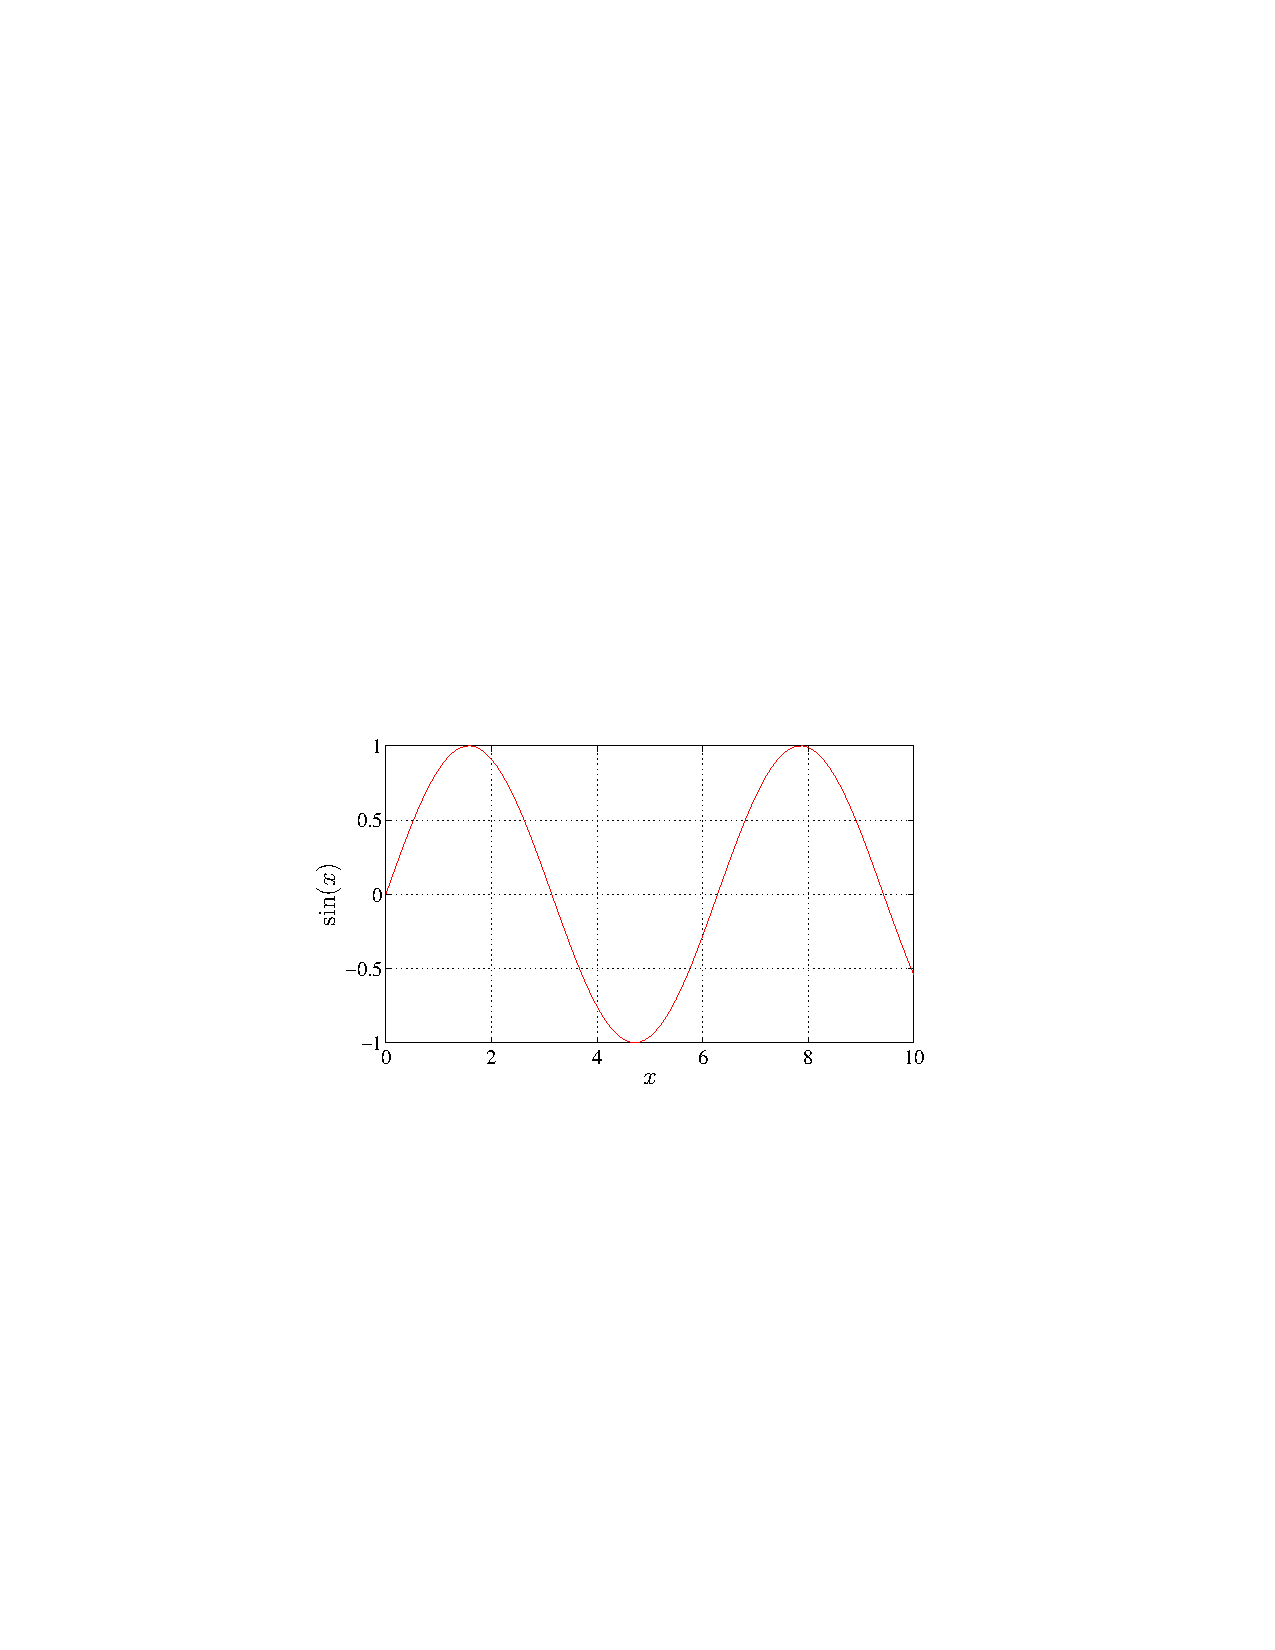
\includegraphics[width=\columnwidth]{fig1a}}
  \caption{Example of a figure with experimental results.}
  \label{fig:results}
\end{figure}

\section{Equations}
\label{sec:equations}

Equations should be placed on separate lines and consecutively
numbered with equation numbers in parentheses flush with the 
right margin, as illustrated in (\ref{eqn:wave_equation}) 
that gives the homogeneous acoustic wave equation in
Cartesian coordinates \cite{eWilliams1999},
\begin{equation}
  \label{eqn:wave_equation}
    \Delta^2p(x,y,z,t)-
    \displaystyle\frac{1}{c^2}\frac{\partial^2p(x,y,z,t)}{\partial t^2}=0,
\end{equation}
where $p(x,y,z,t)$ is an infinitesimal variation of acoustic 
pressure from its equilibrium value at position $(x,y,z)$ and 
time $t$, and where $c$ denotes the speed of sound.

Symbols in your equation should be defined before the equation 
appears or immediately following.  Use (1), not Eq. (1) or 
equation (1), except at the beginning of a sentence:  
``Equation (1) is ...''



\section{FOOTNOTES}
\label{sec:foot}

Use footnotes sparingly (or not at all!) and place them at 
the bottom of the column on the page on which they are 
referenced. Use Times 9-point type, single-spaced. To 
help your readers, avoid using footnotes altogether and
include necessary peripheral observations in the text 
(within parentheses, if you prefer, as in this sentence).


\section{REFERENCES}
\label{sec:ref}

List and number all bibliographical references at the end 
of the paper. The references should be numbered in order 
of appearance in the document. When referring to them in 
the text, type the corresponding reference number in 
square brackets as shown at the end of this sentence 
\cite{cJones2003}, \cite{aSmith2000}. For \LaTeX\ users, 
the use of the Bib\TeX\ style file IEEEtran.bst is 
recommended, which is included in the \LaTeX\ paper 
kit available from the workshop website \cite{waspaa17web}.

\section{ACKNOWLEDGMENT}
\label{sec:ack}

The preferred spelling of the word acknowledgment in 
America is without an ``e'' after the ``g.'' Try to avoid 
the stilted expression, ``One of us (R. B. G.) thanks ...''
Instead, try ``R.B.G.\ thanks ...''  Put sponsor 
acknowledgments in the unnumbered footnote on the first page.

% -------------------------------------------------------------------------
% Either list references using the bibliography style file IEEEtran.bst
\bibliographystyle{IEEEtran}
\bibliography{refs17}
%
% or list them by yourself
% \begin{thebibliography}{9}
% 
% \bibitem{waspaa17web}
%   \url{http://www.waspaa.com}.
%
% \bibitem{IEEEPDFSpec}
%   {PDF} specification for {IEEE} {X}plore$^{\textregistered}$,
%   \url{http://www.ieee.org/portal/cms_docs/pubs/confstandards/pdfs/IEEE-PDF-SpecV401.pdf}.
%
% \bibitem{PDFOpenSourceTools}
%   Creating high resolution {PDF} files for book production with 
%   open source tools, 
%   \url{http://www.grassbook.org/neteler/highres_pdf.html}.
%
% \bibitem{eWilliams1999}
% E. Williams, \emph{Fourier Acoustics: Sound Radiation and Nearfield Acoustic
%   Holography}. London, UK: Academic Press, 1999.
% 
% \bibitem{ieeecopyright}
%   \url{http://www.ieee.org/web/publications/rights/copyrightmain.html}.
%
% \bibitem{cJones2003}
% C. Jones, A. Smith, and E. Roberts, ``A sample paper in conference
%   proceedings,'' in \emph{Proc. IEEE ICASSP}, vol. II, 2003, pp. 803--806.
% 
% \bibitem{aSmith2000}
% A. Smith, C. Jones, and E. Roberts, ``A sample paper in journals,'' 
%   \emph{IEEE Trans. Signal Process.}, vol. 62, pp. 291--294, Jan. 2000.
% 
% \end{thebibliography}


\end{sloppy}
\end{document}
